\subsubsection{Concept}
A neural network is grown in a \textit{micro electrode array} which allows the
neurons to be interfaced with using electrical stimuli in order to control a
robot as shown in \ref{fig:cyborg_idea}.
Building on the theoretical groundwork described in the background, the neural
network is used as a reservoir which is fed sensory input from a robot.
A somewhat subtle but very important consequence of utilizing reservoir
computing is that the neural network does not directly control the robot, it
simply acts as a classifier which responds to the input, and the resulting
dynamics is interpreted by a computer as an action for the robot.
This distinction has little practical consequence for the cyborg, but it offers
an interesting clue into the inner workings of sentience.
\begin{figure}[h!]
    %\centering
    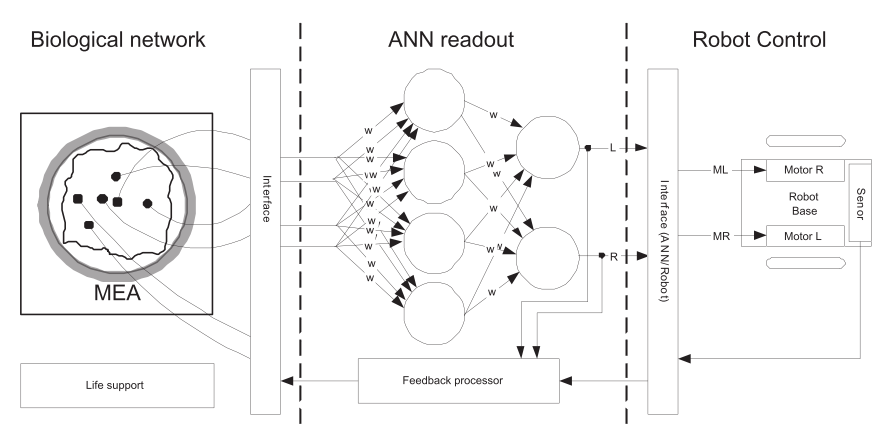
\includegraphics[width=\linewidth]{images/cyborg_overview.png}
    \caption{The gist of it..}
    \label{fig:cyborg_idea}
\end{figure}
\subsubsection{Platform}
Providing an interface between neurons and a computer allows using neural
network for computation, however it is impractical to move the neural cultures
outside of the laboratory.
The practical, yet thought provoking\footnote{For brevity the
  philosophical implications is left as an exercise to the reader.} solution is
using a TCP/IP network protocol such that the neuron culture may be interfaced with any
robot or simulator without leaving the laboratory.
Similar network architectures have been implemented, in
\cite{li_application_2015} a neuron culture is used to control a simple wall
avoiding robot, \#\# something about the shortcomings of this paper? \#\#.
\#\# mention the actual NTNU cyborg here! \#\#
\subsubsection{Growing NIV}
% \begin{enumerate}
% \item[ayy] vise spikes\\
% \item[lmao] pacemakers\\
% \end{enumerate} 
\subsubsection{Current state?}
\begin{figure}[h!]
    %\centering
    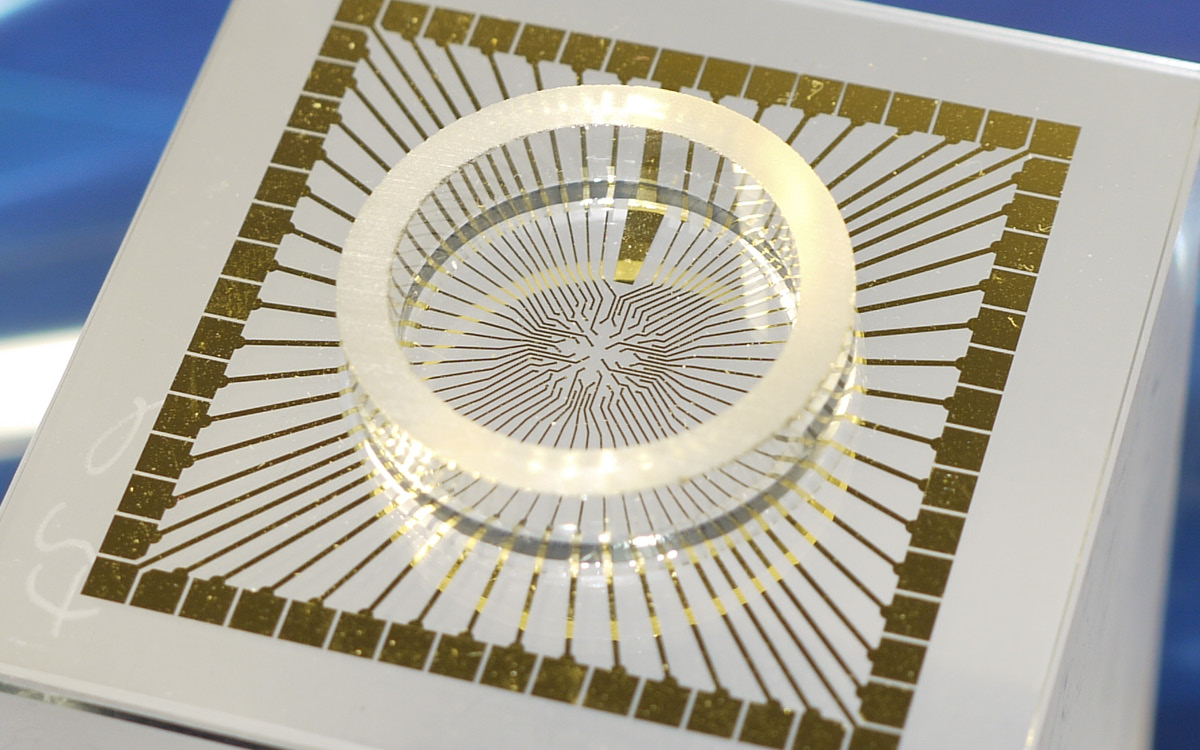
\includegraphics[width=\linewidth]{images/MEA.jpg}
    \caption{A generic MEA}
    \label{fig:generic_MEA}
\end{figure}

\begin{figure}[h!]
    %\centering
    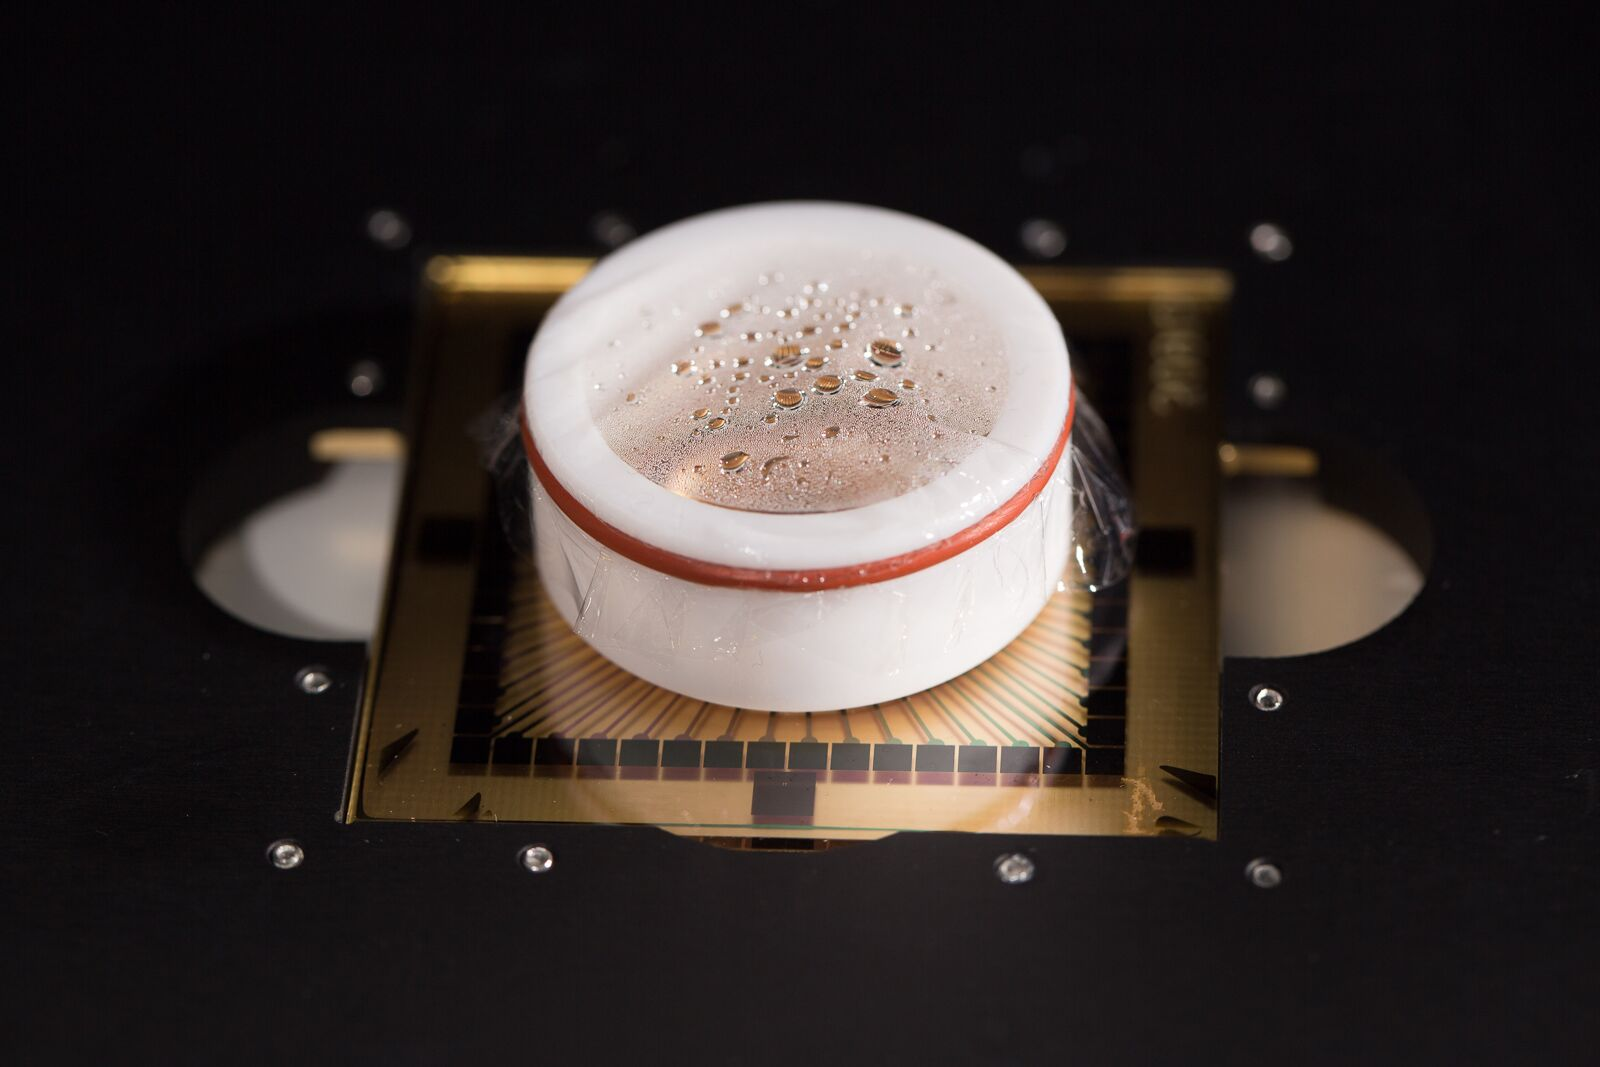
\includegraphics[width=\linewidth]{images/st-olavs-mea.jpg}
    \caption{A MEA with a live culture, photographed by Kai}
    \label{fig:st_olav_MEA}
\end{figure}
\begin{figure}[h!]
    %\centering
    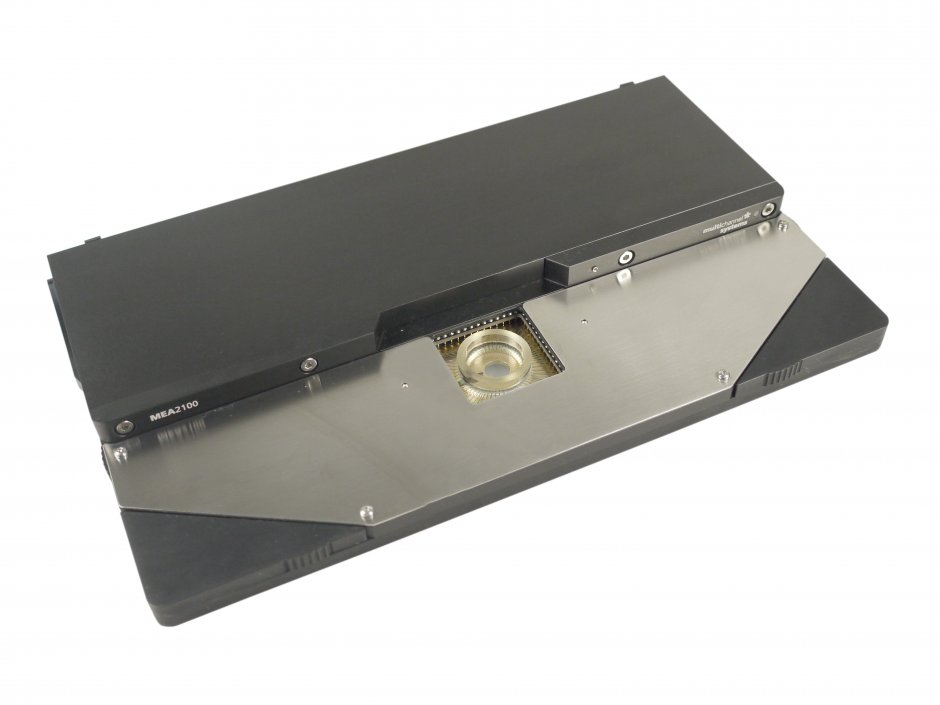
\includegraphics[width=\linewidth]{images/MEA2100-HS60.jpg}
    \caption{The headstage}
    \label{fig:headstage}
\end{figure}
\begin{figure}[h!]
    %\centering
    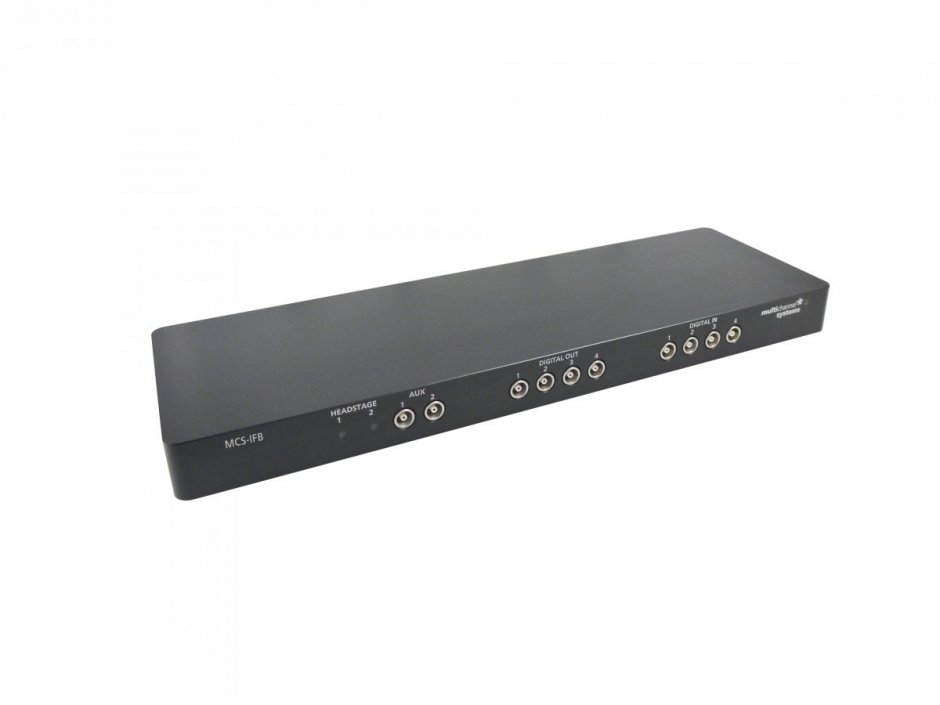
\includegraphics[width=\linewidth]{images/MCS-IFB.jpg}
    \caption{The MCS interface board}
    \label{fig:neuron_anatomy}
\end{figure}
%%% Local Variables:
%%% mode: latex
%%% TeX-master: "../main"
%%% End:
